\section{The automatic bridge}\label{sec:framework}
\ivano{descrizione completa del bridge senza dettagli}
\marco{da sistemare la posizione delle immagini, dopo che saranno finiti i paragrafi precedenti. e completare l'ultimo capoverso, quello che dipende dall'immagine. Per il resto, salvo altre considerazioni "SOLO" da revisionare}


The concept of bridge is used to denote the capability of interoperability between the UML approach and the DSL one. When a corresponding bridge is available for a metamodel and a corresponding profile, it is possible to produce automatically an UML profiled model from a model conforming to the metamodel in question and conversely. In our project we implement a bridge between the metamodels, either between models. The resulting artifacts of the bridge are: a metamodel which represents the profile we are about to translate,  automatically generated transformations which bridge a UML model conforming the profile in question and a model conforming to the brand new generated metamodel.
\begin{figure}[htbp]
	\centering
		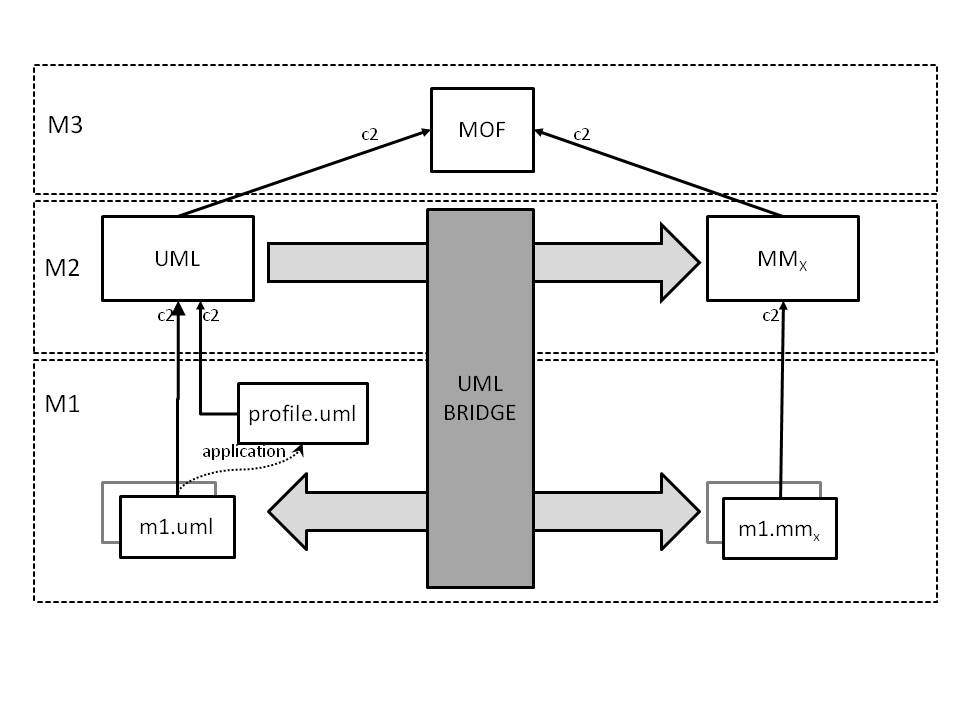
\includegraphics[width=1.00\textwidth]{figures/Diapositiva1.JPG}
	\caption{An overall view of the bridge}
	\label{fig:Diapositiva1}
\end{figure}
In the below figure,  source models are white, representing the input artifacts to be transformed, target models are red, to denote that they are automatically generated. The yellow shapes denote the bridge engine. As it can be noticed, the bridging procedure is split in two phases: the first one, the yellow ellipse in figure, works at the metamodeling level by generating a metamodel which is the representation of the profile (and the UML metamodel); the second phase, the yellow arrow in figure, works at the modeling level by automatically generating transformations from a UML model which has applied a profile to a model which is conform to the brand new generated metamodel.

The resulting metamodel can be considered a union of the UML metamodel (copied in the target one by means of an ad-hoc trasformation superomposed to our one) and the metamodel described in the profile model. We propose a further optimization to our tool which lets the developper to reduce the size of the UML metamodel imported in the target one.

In the following we will show the bridge behaviour at the metamodeling level and at the modeling one. In the end we will show the procedure we propose to slice the obtained metamodel.

\subsection{The bridge at the metamodeling level}\label{sec:metamodelLevel}
\ivano{livello meta con esempietto}

At the metamodeling level the bridge takes as input the UML metamodel and the profile. As shown in the figure \ref{fig:Diapositiva1}, it generates a metamodel by coping the UML metamodel in ECORE formalism, and by adding futher constructs which represent the elements in the profile.  The figure \ref{fig:Diapositiva1} represents a UML profile translated into an EMF metamodel. All the UML metamodel elements are in the target metamodel, all the profiled elements (stereotypes and further data types) are represented in the target metamodel. The extension mechanism of a stereotype and its metaclass is represented by means of a binding mechanism. Every super class has a reference to the eventual stereotype.
\begin{figure}[htbp]
	\centering
		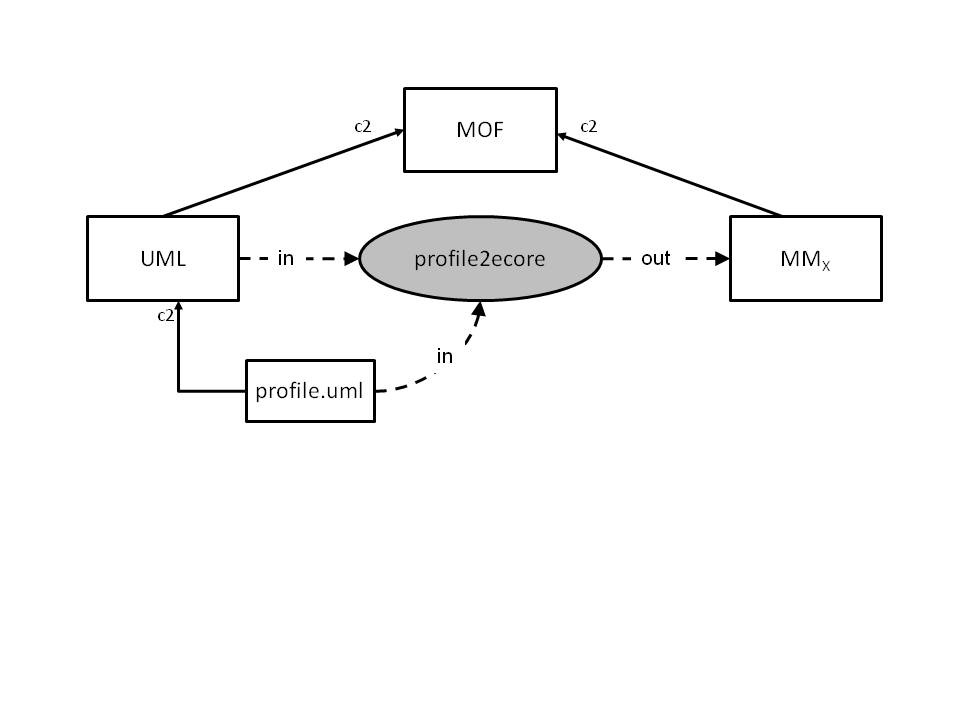
\includegraphics[width=1.00\textwidth]{figures/Diapositiva2.JPG}
	\caption{The bridge at the metamodeling level}
	\label{fig:Diapositiva2}
\end{figure}
In the figure \ref{fig:Diapositiva1} we show the behaviour of our approach. We have a stereotype \emph{MyStereotype2} which extends two metaclasses. By means of the superimposed  transformation we copy the UML metamodel, and we enrich it by adding extension attributes to every metaclasses which has been extended in the profile. The bridge, instead, creates a brand new element bounded with a composition relationship with the metaclasses it extends. In this scenario we have \emph{MyStereotype1} linked to the \emph{Class} metaclass and \emph{MyStereotype2} linked both to \emph{Class} and to \emph{Port}. As you can see in the fgure the classes of the UML metamodel are extended in the target metamodel since they own their attributes plus an extension extra-attribute which binds them to each stereotype.

\subsection{The bridge at the modeling level}\label{sec:modeLevel}

\ivano{livello modello con esempietto}

At the modeling level the bridge automatically generates transformations which bridge a profiled model in a model conforming to the brand new generated metamodel.
\begin{figure}[htbp]
	\centering
		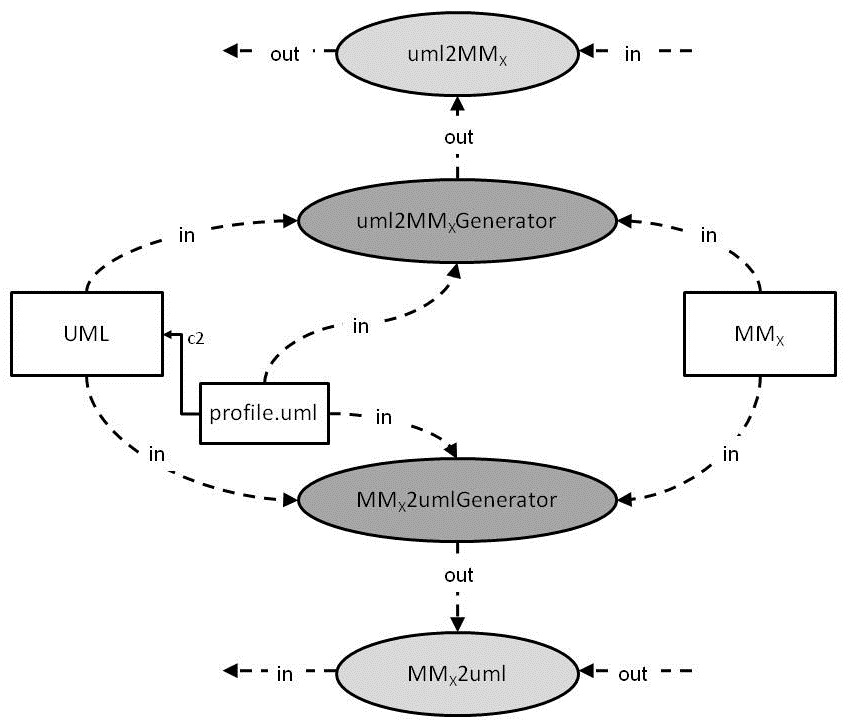
\includegraphics[width=1.00\textwidth]{figures/Diapositiva3.JPG}
	\caption{The bridge at the modeling level}
	\label{fig:Diapositiva3}
\end{figure}
As shown in figure \ref{fig:Diapositiva3}, the transformation generates a transformation at the modeling level in three phases: in the first one we generate rules to transofrm UML metaclasses into EMF ones; in the second phase we generate new rules to transform stereotype�s applications into metaclasses�instances representing the stereotype in the target metamodel; in the last phase we generate imperative code, inserted at the end of every rules generated in the fist phase, to trigger the rules obtained in the second phase. The result is a transformation able to bridge a profiled model in a model conforming to the corresponding brand new genarated metamodel.

By executing this brand new transformation we complete the bridge from UML profiling to EMF metamodeling. As example we use the same scenario of the previous paragraph - modeling level. The model element 
\marco{... bla bla bla}

\section{Slicing the obtained metamodel}\label{sec:slicing}
\ivano{descrizione dello slicing dal punto di vista tecnico}